\chapter{Introduction}\label{chapter:introduction}
Cancer remains one of the most formidable challenges in the realm of health and medicine, causing a quarter of all deaths in the UK \cite{noauthor_cancer_2015}.
Despite advances in cancer research, the survival rates for many cancers remain low, with the disease being an increasing burden on healthcare
systems \cite{noauthor_financial_nodate}. The disease's heterogeneity, both within and between patients, is a major obstacle to effective treatment. Understanding the
underlying evolutionary processes driving this heterogeneity is crucial to developing new treatments and improving patient outcomes.
While having a comprehensive mathematical theory of cancer evolution may not be feasible, concrete mathematical models can provide valuable insights into the
disease's dynamics. To this end, I consider different approaches to modelling cancer evolution, which includes the use of phylogenetic
trees and agent-based models. Further, I employ methylation data to verify the accuracy of the models using Approximate Bayesian Computation (ABC).\par
Trees as a mathematical object have found use in a variety of fields, of which biology is my main focus. However, I have found
interesting links to methods in computer science via information theory.
In chapter \ref{chapter:trees}, I expand upon three points. First, I further establish $J^1$ as a
universal index of tree balance through connections with data structures in computer science. Second, I derive
upper bounds on the error of the expected value approximations for the Yule process and the uniform model.
Finally, I investigate the minimal values of $J^1$ in important special cases,
with special emphasis on the large tree limit. \par
In chapter \ref{chapter:trajectories}, I employ the index $J^1$, along with two other tree shape indices, to
test to what degree one can differentiate between different evolutionary regimes in cancer by only relying
tree shape indices. These results are compared to a new, more comprehensive system of tree shape indices \cite{noble_new_2023}
which further generalised the concepts of diversity, evenness and richness. These results lay the groundwork for
future analysis of cancer tree data.\par
In chapter \ref{chapter:methdemon}, I introduce a tailor-made model for simulating a specific type of molecular data, methylation arrays, obtained from
multi-site sequencing of colorectal cancer. I show that the model is able to recapitulate the patterns observed in the
data and that it can be used to infer the evolutionary history of the tumour. I further explore how the model can be expanded
for more general use due to its modular design. I also demonstrate an approximate Bayesian computation workflow for inferring
the parameters of the model from data, and discuss the choice of summary statistics and the performance of the ABC algorithm.\par
In chapter \ref{chapter:methylation}, I use the new agent-based modelling framework to infer the evolutionary history of
$10$ colorectal cancer samples. Additionally, using tree shape indices, I compare trees of the inferred branching process in the data to the trees
generated in the simulation. This provides an additional tool for validating the model and the inference process. I also
explore the potential of using the model for predicting the future evolution of tumours, and discuss the limitations of the
workflow for this specific use case.\par


\section{Mathematical oncology}
\subsection{Introduction}
Cancer emergence and progression is an evolutionary process \cite{nowell_clonal_1976, merlo_cancer_2006}.
This statement is now widely accepted, and the applications of quantitative methods found in evolutionary
biology in cancer research are numerous \cite{rockne_2019_2019, yin_review_2019, kourou_applied_2021}.
The, now well established, area of mathematical oncology is informed by clinicians, computer scientists,
mathematicians of all flavours, and biologists alike \cite{bull_hallmarks_2022}, which has led to a rapid
development of more specific avenues of research spanning from the initiation of the disease
\cite{paterson_mathematical_2020} to the optimisation of therapy protocols
\cite{west_survey_2023}. This is a perfect reflection of the complexity
of the disease itself, as its rapid evolution, heterogeneity and constraints on
how much information one can obtain from a patient take
the combined efforts of thousands of scientists. Mathematics plays its own role in this effort, providing
a common language through rigour and methods development, and frameworks for the interpretation of data.

\subsection{Mathematical models of tumour evolution}
The specifics of tumour evolution are complex as, while deterministic equations may capture the evolutionary
dynamics of a cohort of tumours, the individual tumour's evolutionary history is stochastic
\cite{werner_deterministic_2013}. This only adds to the issue of how the surrounding tissue \cite{west_normal_2021}
and the tumour's own spatial organisation will affect its progression \cite{noble_spatial_2022}. Therefore,
existing models of tumour evolution have had to incorporate both general, large-scale processes and
sometimes molecular level events to be able to claim progress towards personalised cancer care informed
by quantitative models \cite{yin_review_2019}. \par
As mentioned earlier, the applications of mathematics in oncology are diverse. Thus, my focus over the course
of this PhD has been on modelling tumour evolution and progression from its early stages up to and excluding
treatment. This makes the problem more of an exercise in populatin dynamics than strict oncology, as underlying
assumptions of such models tend to focus less on the microenvironment impact and more on how mutations accumulate
and spread in the tumour. A good example of one such model is the Big Bang model of tumour growth \cite{sottoriva_big_2015}.
Informed by multi-site sequencing, the authors' hypothesis was that colorectal cancer evolves neutrally after an initial
period of rapid expansion and selection. Much like cosmic microwave background radiation is unevenly distributed across the
observable universe, they observed an asymmetrical distribution of mutations across the tumour spheroid.
This inspired a spatial branching process model based on gland fission, with each tumour gland approximated to
rapid fixation in the event of a driver mutation, which showed good agreement with the data. A follow-up paper \cite{williams_identification_2016}
ignited a debate on neutral evolution in exponentially growing tumours within the community
\cite{tarabichi_neutral_2018, mcdonald_currently_2018, heide_reply_2018, bozic_measuring_2019}.
However, theoretical considerations of the two-level model compared to the neutral model did, in fact,
show that it is possible to distinguish the two based on mutation frequency spectra \cite{tung_signatures_2021}.\par
One would be remiss, however, to only focus on models explicitly designed for cancer. The abstract nature of
mathematical modelling has allowed for the transfer of knowledge between fields, with models developed for
other purposes being applicable in cancer. General models which are more easily tested on, for example, bacterial
populations \cite{fusco_excess_2016, schreck_impact_2023} can be adapted to cancer, as the underlying principles
of evolution are the same. But digging even deeper, the underlying model of boundary growth dates back to the
Eden model of crystal growth \cite{eden_two-dimensional_1961}. Among similar examples are uses of the
Fisher-Kolmogorov-Petrovsky-Piscounov equation in ecology and its modifications for the study of the spread
of mutations in populations with a constant size \cite{houchmandzadeh_fisher_2017} as well as growing populations
\cite{wodarz_mutant_2020}.
Further, the use of phylogenetic trees and methods in cancer is an emerging field
introduced in the following section and expanded upon in chapters \ref{chapter:trees} and \ref{chapter:trajectories}.


\section{Trees and their applications}

\subsection{Introduction}
In the most general sense, a tree is a connected graph with no cycles. In this thesis, when a tree is
mentioned, I refer to a rooted tree, as formally defined in section \ref{sec:preliminary_defs}.
Trees have found use in a variety of fields, including computer science, biology, and linguistics.
In computer science, trees are used to represent hierarchical data structures, such as file systems \cite{nievergelt_binary_1974}
or the structure of a program's syntax \cite{knuth_semantics_1968}, an approach that computer scientists
share with linguists \cite{chomsky_syntactic_1957}. The concept of search trees, dating back to the mid 20th century,
revolutionised the field of computer science with applications in information retrieval in the form of
binary search trees and self-balancing trees \cite{nievergelt_binary_1972, knuth_art_1997}. In evolutionary biology,
one of the earliest appearances of trees dates back to the 19th century, when Charles Darwin used them to represent the evolutionary
relationships between species. Phylogenetic trees have over time become a key tool in analysing the
lineages of species, viral mutations, and cancer evolution. By investigating quantitative summaries of different properties
of tree shapes, one can gain insight into the underlying processes driving the evolution of species \cite{mooers_inferring_1997}
or cancer \cite{scott_inferring_2018, noble_spatial_2022}. However, most of the inference work so far has been performed
using methods which are not necessarily rooted in sound mathematical theory, but are rather based on heuristics \cite{omeara_evolutionary_2012}.
Specifically, measures of tree balance suffer from a lack of a common framework, with at least $19$ different metrics available
in literature \cite{fischer_tree_2021}, and few of them being directly comparable. Also, due to the divergent terminology and
interest in the use of trees as a tool, there is scarce literature on the transfer of knowledge between the fields of computer science
and biology, with certain results being rediscovered nigh on half a century later, as discussed in section \ref{sec:trees_compsci}.

\subsection{Quantifying tree balance}
In a recent paper \cite{lemant_robust_2022}, Lemant and Noble proposed a new robust, universal index, $J^1$, for quantifying the
balance of rooted trees with arbitrary node degree and size distributions. This index is based on
Shannon entropy and favours even distributions of node sizes. By generating large numbers of random trees
using the alpha-gamma model, I showed that $J^1$ is robust, in the sense
that it is insensitive to small changes in node sizes and to the removal of small nodes (figure \ref{fig:robustness}B, C).
Noble and I further showed that this index unites and generalises two of the most
popular prior approaches to quantifying tree balance in biology, the Colless index and the Sackin index.
Applied to evolutionary trees, $J^1$ outperforms conventional tree balance indices as a summary statistic
for comparing model output to empirical data \cite{noble_spatial_2022}.\par
Given any tree shape index, an important task is to obtain its expected and extreme values under standard
tree-generating processes, which can then be used as null-model reference points. In \cite{lemant_robust_2022},
Noble and I obtained analytical approximations to the expected values of $J^1$ under the Yule process and the uniform
model, and I tested their accuracy numerically for trees with up to $128$ leaves (figure \ref{fig:robustness}A). In the
same study, Noble and I proved that caterpillar trees minimise $J^1$ among bifurcating trees but not when larger
outdegrees are permitted.\par

\begin{figure}[h]
    \centering
    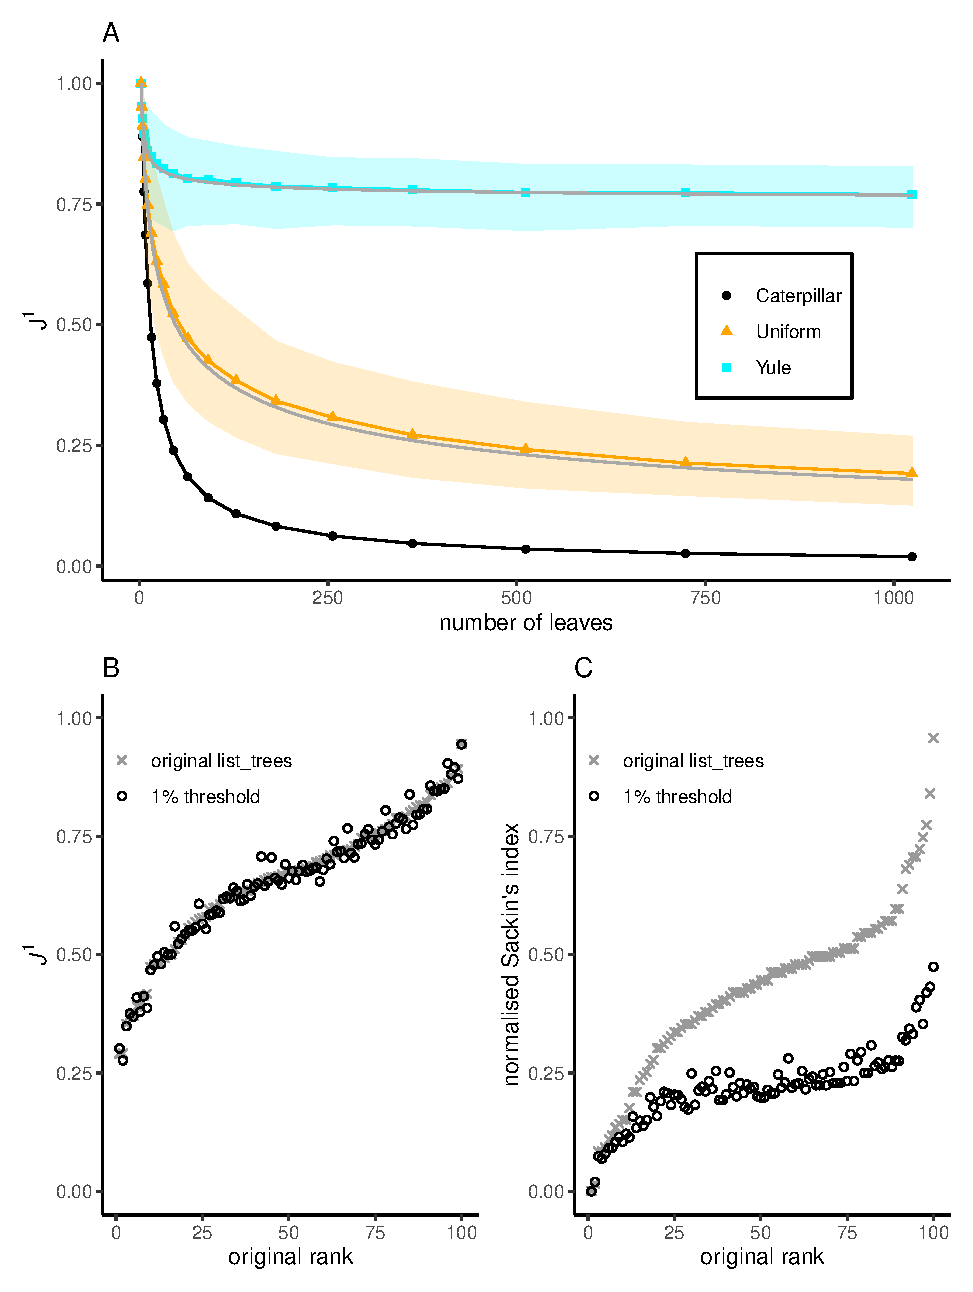
\includegraphics[width=0.82\textwidth]{Chapter_1/figures/old_j1_paper_figure.pdf}
    \caption{\textbf{A} $J^1$ values for trees generated under the Yule process and
    the uniform model. Solid grey curves represent the approximate expected values, and
    the dashed lines the $5$th and $95$th percentiles. \\
    \textbf{B} $J^1$ values for $100$ random
    trees on $16$ leaves using the alpha-gamma model, with $\alpha\sim \text{Unif}(0,1)$
    and $\gamma\sim \text{Unif}(0,\alpha)$. The values were
    calculated before and after applying a $1\%$ population threshold, i.e. removing all leaves
    with sizes smaller than $0.01$ times the total population.\\
    \textbf{C} Normalised Sackin index values for the same trees as in \textbf{B}.}
    \label{fig:robustness}
\end{figure}
\clearpage


\section{Agent-based modelling in oncology}

\subsection{Introduction}
Agent-based models (ABMs) are a class of computational models that simulate the actions and interactions of individual
agents within a system. These agents can represent anything from cells in a tissue to animals in an ecosystem. ABMs
are particularly useful in cancer research, as they can capture the complex interactions happening on the microscale in
cancer. Spatial agent-based models (SABMs) are a subclass of ABMs that incorporate spatial information into the
simulations. This is particularly useful for modelling solid tumours as it allows for the simulation of things like
the spatial heterogeneity of the tumour microenvironment and the effects of spatial constraints on tumour growth.
A strength of ABMs is that they can be as simple or as complex as the researcher needs them to be \cite{colyer_seven-step_2023}.
However, therein lies their weakness, as oversimplification of a model can lead to rapid loss of its utility in
capturing the behaviour of a complex system such as cancer. On the other hand, a model that is too complex, and
attempts to include everything from epigenetic mutations to the effects of the immune system on the tumour, is likely
too computationally expensive to be useful for modelling a tumour of reasonable size. This is an organic demonstration
of many a researcher's favourite saying \textit{all models are wrong, but some are useful, and some are more useful
than others}. In parsing through the literature and developing a new model of my own, I have also been influenced
by an alternative wording of this, that is \textit{the best model is its own worst enemy}, by mathematical biologist Philip
Maini \cite{maini_talk_2023}. My
interpretation is that a good model should address the questions it was designed to answer, but also open up new
ones which require further investigation, improvements, and research. For example, one can use the \texttt{demon-warlock}
framework \cite{bak_warlock_2023} to simulate the evolution of a tumour in space and draw conclusions on how
spatial organisation will impact intratumour heterogeneity or patient outcomes \cite{noble_when_2020, noble_spatial_2022}.
However, the model does not address the impact of the immune system, spatial heterogeneity in the microenvironment,
or the effects of therapy without further modifications. Alternatively, one may want to include diffusion of
nutrients and waste products in the model, or the effects of hypoxia on the tumour cells. Tools that would be
appropriate for such tasks are, for example, HAL \cite{bravo_hybrid_2020} or PhysiCell \cite{ghaffarizadeh_physicell_2018},
but they are not ideal either as simulating a realistically-sized tumour with these models is prohibitively expensive
in terms of computational resources. Thus, my preferred approach is to develop a purpose-made model which is
informed by the literature and the data, and which has ample room for future expansion and improvement.

\subsection{The \texttt{demon-warlock} framework}
In a recent paper \cite{bak_warlock_2023}, a new agent-based model for simulating the evolution of a tumour in space
was introduced. The model is designed to be versatile and able to simulate a wide range of
spatial configurations and evolutionary properties of cancer. Spatially, the model is based on a 2D grid, where
each grid cell represents a deme, that is a spatially homogeneous population of cells. Each cell in the model
belongs to a genotype, a unique identifier based on the cell's mutations, and a driver genotype, which differentiates
itself from the genotype by not taking into account passenger mutations. Cell migrations in the tumour have multiple
modes, including invasion of tissue and other demes, and deme fission. The latter allows for the simulation of
tumours with a glandular structure, such as colorectal cancer. Events in the model are scheduled according to the
Gillespie algorithm, with the event hierarchy shown in figure \ref{fig:demon_events}. As the model was written
predominantly in plain C, it is highly efficient considering the complexity of the simulations it can run. An
accompanying R package, \texttt{demonanalysis}, is available for the analysis and visualisation of the model's
output, e.g. figure \ref{fig:demonanalysis_example}. \par
Despite the model's versatility, it is not without its limitations. In its current form, it is not feasible to
simulate tumours larger than a few million cells. This leaves out the possibility of simulating realistically-sized
glandular tumours which can contain a few million glands containing thousands of cells each at the time of diagnosis.
Furtermore, as the main limitation of the model's scalability is tied to the inherent inefficiency of generating
random numbers, it is not well-suited to simulating neutral stochastic markers, such as fluctuating methylation
clocks \cite{gabbutt_fluctuating_2022}. This is further discussed in section \ref{section:old_famework}.

\begin{figure}[h]
    \centering
    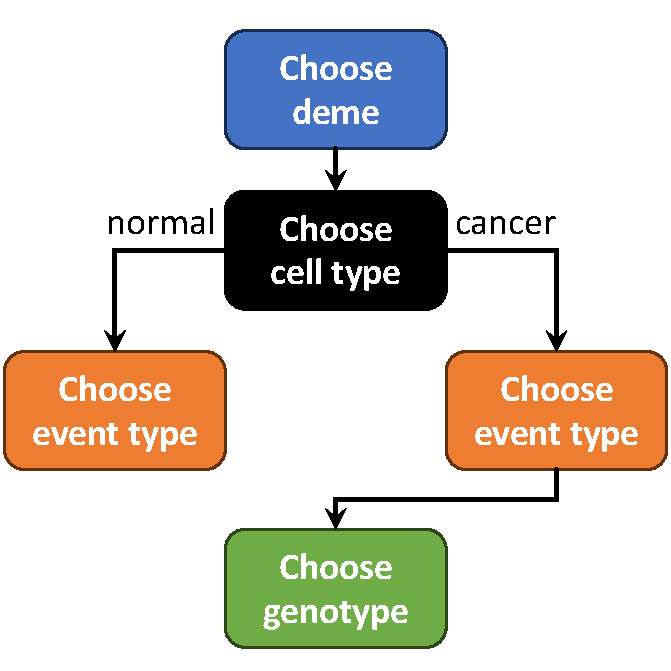
\includegraphics[width=0.75\textwidth]{Chapter_1/figures/demon_hierarchy.pdf}
    \caption{Event hierarchy in the \texttt{demon-warlock} framework. Figure reproduced from \cite{bak_warlock_2023} with
    the authors' permission.}
    \label{fig:demon_events}
\end{figure}

\begin{figure}[h]
    \centering
    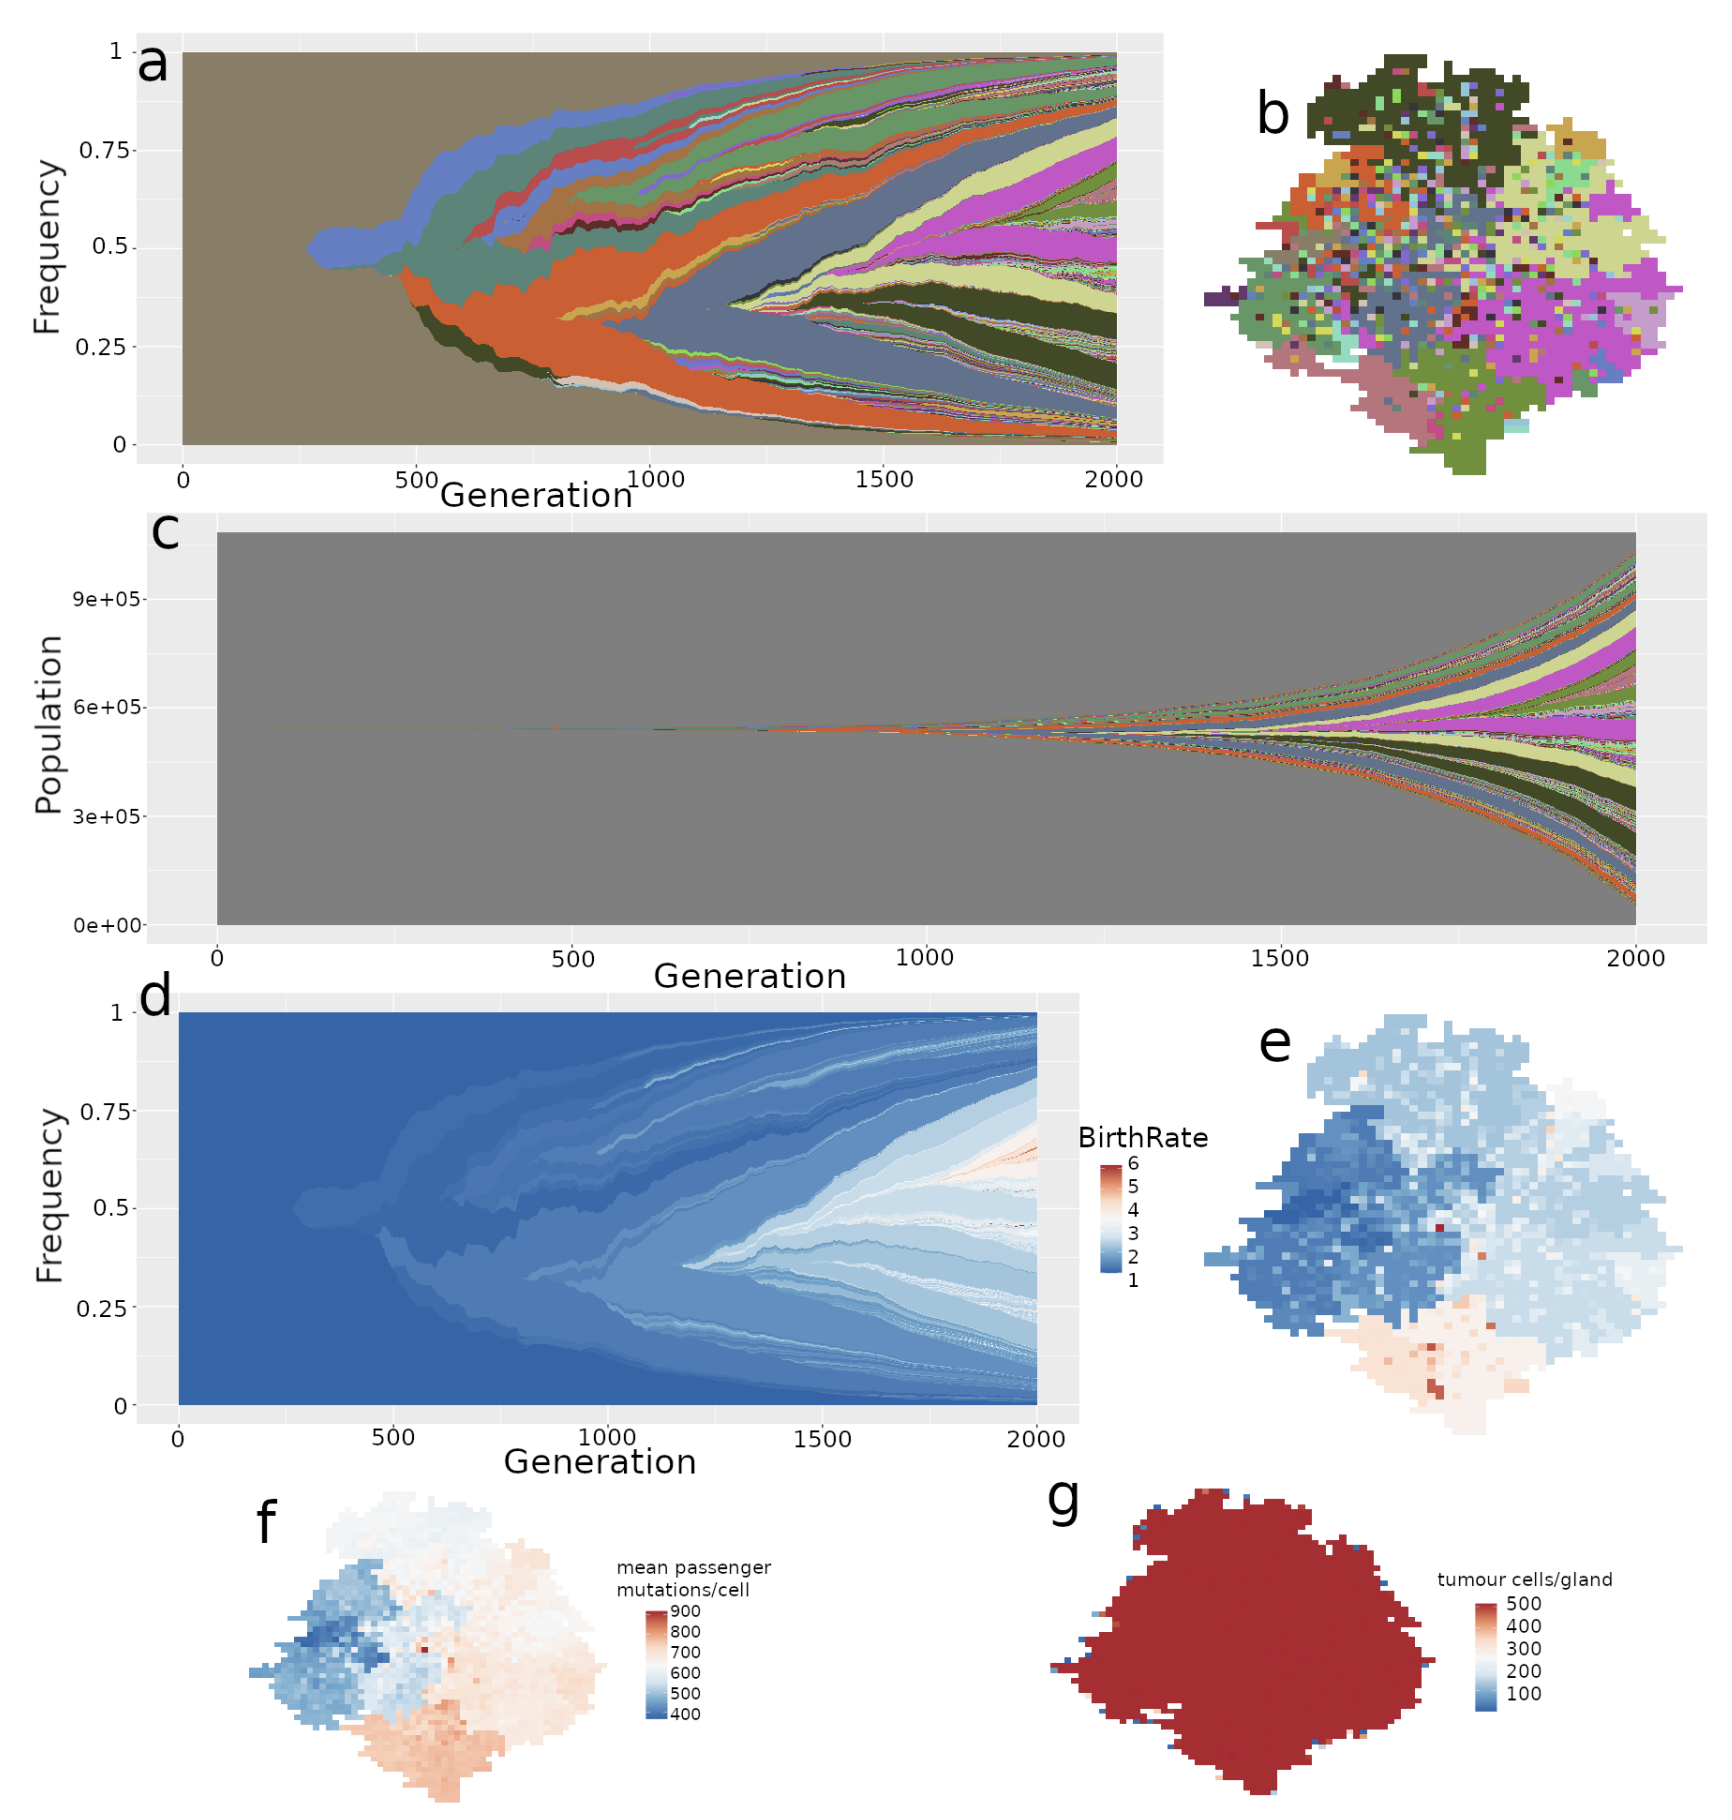
\includegraphics[width=\textwidth]{Chapter_1/figures/demonanalysis_example.png}
    \caption{Example output from \texttt{demon}, visualised using the \texttt{demonanalysis} package.
    \textbf{a} Muller plot of clonal dynamics over time. Each colour represents a clone with a distinct
    combination of driver mutations.
    \textbf{b} Final proportions and spatial plot of clones.
    \textbf{c} Fish plot of clone populations over time using the same colours as in \textbf{a}.
    \textbf{d} Muller plot showing evolution of tumour cell division rate.
    \textbf{e} Final spatial distribution of cell division rates.
    \textbf{f} Final spatial distribution of the mean numbers of passender mutations per cell.
    \textbf{g} Final spatial distribution of the number of tumour cells per gland.}
    \label{fig:demonanalysis_example}
\end{figure}
\clearpage

\section{Likelihood-free inference}
\subsection{Introduction}
To verify whether a model predicts behaviour of the observed system, a common approach is comparing its
output to measurements. The way this is done depends on the complexity of the model and the data. Here
we discuss the general framework of likelihood-free inference, and more specifically the use of Approximate
Bayesian Computation (ABC). \par
Models based on differential equations can be compared to data using likelihood-based methods. In the
frequentist tradition, the likelihood function is used to estimate the parameters of the model under the
assumption that there is a correct, or ``true" value of those parameters. An alternative approach is
Bayesian statistics, which uses random variables ($\theta$) to represent the uncertainty in the parameters. The
distribution of these random variables before observing the data is called the prior distribution ($P(\theta)$).
After performing measurements in the system and obtaining data ($D$) which has an associated likelihood function
($P(D|\theta)$), the prior distribution is update to the posterior distribution ($P(\theta|D$)) using Bayes' theorem
\cite{bayes_essay_1763}:
\begin{equation}
    P(\theta|D) = \frac{P(D|\theta)P(\theta)}{P(D)}
\end{equation}
The likelihood function is thus a key component of Bayesian statistics, quantifying the probability of observing
the data given the parameters of the model. However, its greatest asset is also its greatest weakness. Depending
on the complexity of the model and the data, the likelihood function can be difficult or impossible to calculate
analytically, or can be too computationally expensive to calculate numerically. This is especially true for
stochastic models, such as agent-based models, where the likelihood function is often intractable. \par
In the case of intractable likelihoods, a common approach is to use likelihood-free inference methods, designed
to approximate the posterior distribution without the need to calculate the likelihood function. These methods
rely on the generation of simulated data from the model, and the comparison of these simulations to the observed
data. Instead of calculating the likelihood fucntion, these methods often involve a process of simulation and
rejection. A common drawback of likelihood-free inference methods is that they can be computationally expensive,
as they often require a large number of simulations to obtain a good approximation of the posterior distribution.
However, as the computational power of modern computers increases, these methods are becoming more and more
feasible for a wide range of models and data.

\subsection{Approximate Bayesian Computation}
Approximate Bayesian Computation (ABC) is a likelihood-free inference method that has gained popularity in the
last three decades \cite{tavare_inferring_1997, lechevallier_integrating_2010, jagiella_parallelization_2017}.
The basic idea behind ABC is to approximate the posterior distribution of the parameters of a model by comparing
simulated data to observed data. \par
In the most general form of ABC, the algorithm proceeds as follows:
\begin{enumerate}
    \item Sample a set of parameters from the prior distribution, $\hat\theta$.
    \item Simulate data from the model using the parameters.
    \item Compare the simulated data ($\hat D$) to the observed data ($D$) using a distance function, $d(\hat D, D)$.
    \item If the distance between the simulated and observed data is less than a certain threshold $\epsilon$, accept the
    parameters. Otherwise, reject them.
    \item Repeat steps 1-4 until a sufficient number of accepted parameters have been obtained.
\end{enumerate}
The distance threshold must be strictly positive, and is often chosen to be a small value. Alternatively, in the
case of high-dimensional data, the distance function can be replaced by a summary statistic, $S$, which is a function of the
data, i.e. $d'(S(\hat D), S(D))$. \par
ABC does not come without its own set of challenges. As it relies on comparing relevant features of the simulated data to
the observed data, the choice of summary statistic or distance metric is crucial, as it determines how the data is
reduced before the comparison. Fortunately, there are methods for reducing dimensionality of the data which
narrows in on its informative aspects \cite{blum_comparative_2013}.
The choice of the distance threshold is also important, as it determines
the acceptance rate of the algorithm. Setting the threshold too high or too low can lead to biased or inefficient
estimates of the posterior distribution. However, this can be mitigated by using a dynamic threshold, which is
adapted during the course of the algorithm \cite{prangle_adapting_2017}.
Finally, as the algorithm relies on repeated simulations of
potentially complex models. This can require a large amount of computational resources, raising questions about
the method's scalability and practicality. An obvious way to circumvent this is to use a model which is as
lightweight as possible. Even in the case of infinite compute available, one must be mindful of the fact that
the more complex the model, the more complex the inference problem, and the more complex the inference problem,
the more complex the model. This is a feedback loop which can render both the model and subsequent analysis
uninterpretable. Therefore, I believe that the best practice as a mathematician and applied scientist is to abstract
the model enough to be able to draw conclusions from it, but not so much that it becomes uninformative. \par
In chapter \ref{chapter:methdemon}, I introduce a simplified model of colorectal cancer gland fission and
the accompanying ABC workflow. I discuss the choice of summary statistics and the performance of the ABC
algorithm, and subsequently demonstrate the model's utility in inferring the evolutionary history of a tumour
from methylation data in chapter \ref{chapter:methylation}.


\section{Fluctuating methylation clocks}
The concept of the molecular clock is commonplace in molecular evolutionary biology. It is based on the idea that the
rate of evolution of a particular gene or set of genes is constant over time, and can be used to estimate
the time of divergence between species or the time of a particular event in the evolutionary history of a
species. The most famous example of a molecular clock is the mitochondrial DNA clock, which is used to
estimate the time of divergence between species \cite{hasegawa_dating_1985}. The key principle behind molecular
clocks is that closely related species or individual will have more similar sequences than distantly related
ones. This also translates to individual cells in cancer. The issue with using molecular clocks in cancer
is that ``slowly ticking" molecular clocks, i.e. ones with a low mutation rate, are not informative enough
on the timescale of cancer evolution, limiting their utility to cell lineages which diverged too far in the past,
with recent events remaining undetectable. On the other hand, ``fast ticking" molecular clocks can
reveal recent evolutionary events but also have their own limitations, such as independent mutations in the
same site \cite{kuipers_single-cell_2017}. \par
Recently, a new type of molecular clock has been proposed, the fluctuating methylation clock, based on the
observation that the methylation status of certain CpG sites in the genome is heritable but fluctuates
stochastically over time \cite{gabbutt_fluctuating_2022, gabbutt_evolutionary_2023}. A CpG site is a
cytosine nucleotide followed by a guanine nucleotide in the linear sequence of bases along its
5' $\rightarrow$ 3' direction, and is a common site of methylation in the genome. As citosine and guanine
are complementary, each CpG site in the 5' $\rightarrow$ 3' direction has a corresponding pair in the
3' $\rightarrow$ 5' direction. This means that each CpG pair can be in one of three states: both
methylated (homozygously methylated), both unmethylated (homozygously unmethylated), or one methylated
and the other unmethylated (heterozygously methylated). Depending on tissue type, the fluctuating CpG
(fCpG) sites can number somewhere between $1000$ and $2000$, which means each cell has a potentially
unique barcode in its fCpG array. As the array is not constant, with methylations and demethylations
of fCpG sites happening over the course of cell divisions, the authors of the two papers covering fCpGs
so far have been able to reconstruct the evolutionary history of healthy colonic crypts and lymphoid
malignancies with high accuracy. This is a promising development, as sequencing methylation arrays
is a cheaper method than genome sequencing, but may offer finer temporal resolution. In chapter
\ref{chapter:methylation}, I investigate whether multi-site methylation array sequencing can be used
to reconstruct clonal dynamics of colorectal cancer.


\section{Aims}

\subsection{Hypotheses}
\begin{enumerate}
    \item The $J^1$ index can be used, in conjunction with other
        tree shape indices, to differentiate between evolutionary modes in cancer.
    \item SABMs recapitulate molecular data observed in solid tumours (or sth like that)
    \item These methods are useful for inferring the evolutionary history of colorectal cancer based on multi-site
        methylation array sequencing.
\end{enumerate}

\subsection{Aims}
\begin{enumerate}
    \item Calculate or approximate important properties of the $J^1$ index, such as its expected value under
        standard tree-generating processes.
        \begin{enumerate}
            \item Contextualise $J^1$ within the broader field of tree shape indices in biology and computer science.
            \item Investigate extreme and expected values of $J^1$ under standard tree-generating processes.
        \end{enumerate}
    \item Determine the utility of sets of tree shape indices for differentiating between evolutionary modes in cancer.
        \begin{enumerate}
            \item Recapitulate the classification of evolutionary modes in cancer using a set of three tree shape indices.
            \item Extend the discussion to a more interpretable and general system of tree shape indices.
        \end{enumerate}
    \item Extend the fluctuating methylation clock model to multi-site sequencing of solid tumours on the
        example of colorectal cancer.
        \begin{enumerate}
            \item Develop an agent-based model for simulating the evolutionary dynamics of colorectal adenocarcinoma.
            \item Develop an ABC workflow for inferring the evolutionary parameters of the model, specifically the
                gland fission rate, methylation and demethylation rates, driver mutation rate, selective advantage,
                and the effective number of lineages per tumour gland.
            \item Apply the model to colorectal cancer data and compare the inferred phylogenies to the trees generated
                by the model.
        \end{enumerate}
\end{enumerate}
